\subsection{Controlled Validation Results}
\label{subsec:controlled_validation_results}

To validate the framework under reproducible propagation conditions, the first experiment is designed as controlled validation experiment.
For this reason, the framework is tested with two different scenes: free space and an indoor warehouse as shown in Figure \ref{fig:exp1_scenes}.
Free space scene is least obstructed and it is used as a baseline.
Warehouse scene represents the indoor use case where there are multiple reflections and blockages from the warehouse infrastructure.
These two scenes make it possible to observe how the same sensing and beamforming pipeline changes when visibility and clutter change.

\begin{figure}[t]
    \centering
    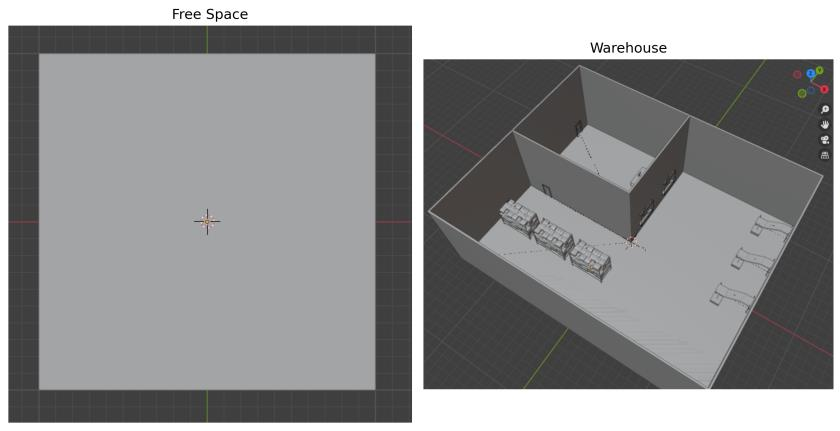
\includegraphics[width=\columnwidth]{images/exp1_scenes.png}
    \caption{Controlled-validation scenes.}
    \label{fig:exp1_scenes}
\end{figure}

Each scene is tested with the same basic procedure so that the differences in the results are caused by scene and ISAC configuration rather than changes in workflow.
The free-space and warehouse use cases use the sinusoidal trajectories of the robots shown in Figure \ref{fig:exp1_trajectories}.
The system is evaluated for $100$ time steps with a $0.2$ seconds interval, providing a $20$ seconds observation window.
At each step, propagation is computed and, when situation awareness is enabled, the sensing module produces detections that are filtered, clustered, tracked, and then used for sensing-informed beamforming.
The baseline does not use ISAC features and performs communication only, while the ISAC variants enable or disable specific functions such as MTI, tracking, beamwidth selection, and propagation depth in order to isolate one part of the proposed pipeline.

\begin{figure}[t]
    \centering
    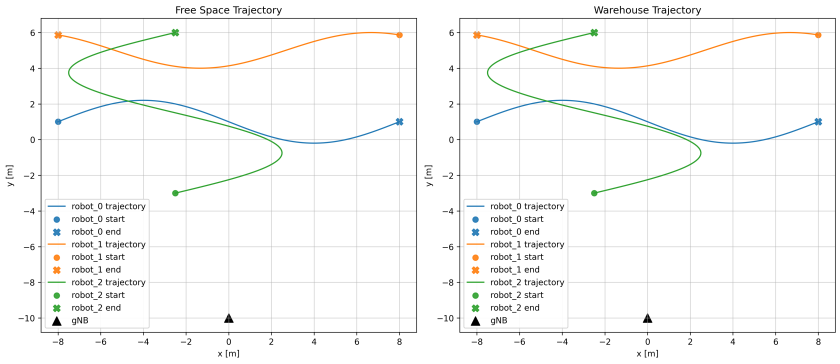
\includegraphics[width=\columnwidth]{images/exp1_trajectories.png}
    \caption{Deterministic robot trajectories used in the controlled
        validation scenes.}
    \label{fig:exp1_trajectories}
\end{figure}

The \texttt{isac\_full} variant test the whole pipeline.
The \texttt{isac\_no\_mti} variant disables only MTI to test whether removing static-reflection suppression affects detection stability.
The \texttt{isac\_narrow} and \texttt{isac\_wide} variants change only beamwidth to compare tighter target focusing against wider coverage under localization error.
The \texttt{isac\_deep} variant increases propagation depth to test whether additional multipath improves sensing or mainly adds clutter.
The \texttt{isac\_no\_tracker} variant disables temporal tracking to test whether raw frame-by-frame detections are sufficient for beamforming.
After each run, the estimated target positions are matched to the known ground truth from the trajectories with the Hungarian algorithm, where unmatched estimates are considered as false positives and unmatched targets are considered as missed detections.

\subsubsection{Free-Space Scene}
\label{subsubsec:controlled_validation_free_space}

The results in Table \ref{tab:exp1_fs_prop} shows that enabling ISAC reduces the mean path loss from $102.39$ dB to the range $84.39$--$86.82$dB.
The mean path delay remains at $54.10$ ns as the mean distance is same for all the variants.
The differences of performance is more observable in received power as in path loss.
Among the tested ablations, \texttt{isac\_wide} achieves the lowest path loss and the strongest received power, which indicates that the wider beam is beneficial when clutter is minimal.

\begin{table}[t]
    \centering
    \caption{Free-space propagation metrics.}
    \label{tab:exp1_fs_prop}
    \footnotesize
    \begin{tabular}{lccc}
        \hline
        Variant           & Path loss [dB] & Delay [ns] & Rx power [dBm] \\
        \hline
        baseline          & 102.39         & 54.10      & $-56.39$       \\
        isac\_full        & 86.30          & 54.10      & $-40.30$       \\
        isac\_no\_mti     & 85.53          & 54.10      & $-39.53$       \\
        isac\_narrow      & 86.82          & 54.10      & $-40.82$       \\
        isac\_wide        & 84.39          & 54.10      & $-38.39$       \\
        isac\_deep        & 85.54          & 54.10      & $-39.54$       \\
        isac\_no\_tracker & 85.43          & 54.10      & $-39.43$       \\
        \hline
    \end{tabular}
\end{table}

The sensing and tracking results in Table~\ref{tab:exp1_fs_sense} follow a similar trend.
The tracking-enabled ISAC variants achieve detection rates between $0.847$ and $0.903$, while their false-positive rates remain close to $0.018$--$0.019$.
Among them, \texttt{isac\_deep} achieves the highest detection rate $0.903$ and lowest missed-detection rate $0.097$, which shows that additional propagation depth can help to detect better but the gain over the other tracked variants is small.
However, the extra computation necessary for deeper propagation does not worth the gain.
The \texttt{isac\_no\_tracker} variant achieves the highest raw detection rate ($0.970$), but it also increases the false-positive rate to $0.176$.
This means that the tracker is useful because it trades raw sensitivity for cleaner detection.

\begin{table}[t]
    \centering
    \caption{Free-space sensing metrics.}
    \label{tab:exp1_fs_sense}
    \footnotesize
    \begin{tabular}{lccccc}
        \hline
        Variant           & Det.  & FPR   & Miss  & Err. [m] & Cont. \\
        \hline
        baseline          & 0.000 & 0.000 & 1.000 & --       & 0.000 \\
        isac\_full        & 0.847 & 0.019 & 0.153 & 1.148    & 0.550 \\
        isac\_no\_mti     & 0.897 & 0.018 & 0.103 & 1.125    & 0.537 \\
        isac\_narrow      & 0.897 & 0.018 & 0.103 & 1.125    & 0.537 \\
        isac\_wide        & 0.897 & 0.018 & 0.103 & 1.125    & 0.537 \\
        isac\_deep        & 0.903 & 0.018 & 0.097 & 1.126    & 0.510 \\
        isac\_no\_tracker & 0.970 & 0.176 & 0.030 & 1.208    & 0.583 \\
        \hline
    \end{tabular}
\end{table}

\subsubsection{Warehouse Scene}
\label{subsubsec:controlled_validation_warehouse}

In the warehouse scene, because of obstacles such racks and partial visibility create the clutter which makes sensing difficult.
The propagation results in Table \ref{tab:exp1_wh_prop} show that ISAC still improves communication, but the gain is smaller than free space case.
With ISAC, mean path loss drops from $109.16$ dB to $94.50$--$101.75$ dB across the ISAC variants.
Like in free space case, \texttt{isac\_wide} is the best in terms of path loss and received power, where it achieves $94.50$ dB path loss and $-48.50$ dBm received power.

\begin{table}[t]
    \centering
    \caption{Warehouse-scene propagation metrics.}
    \label{tab:exp1_wh_prop}
    \footnotesize
    \begin{tabular}{lccc}
        \hline
        Variant           & Path loss [dB] & Delay [ns] & Rx power [dBm] \\
        \hline
        baseline          & 109.16         & 53.95      & $-63.16$       \\
        isac\_full        & 97.90          & 53.95      & $-51.90$       \\
        isac\_no\_mti     & 97.39          & 53.95      & $-51.39$       \\
        isac\_narrow      & 101.75         & 53.95      & $-55.75$       \\
        isac\_wide        & 94.50          & 53.95      & $-48.50$       \\
        isac\_deep        & 97.44          & 53.95      & $-51.44$       \\
        isac\_no\_tracker & 98.52          & 53.95      & $-52.52$       \\
        \hline
    \end{tabular}
\end{table}

The sensing results in Table~\ref{tab:exp1_wh_sense} show that sensing in the warehouse scene is more difficult than in free space.
The tracked variants of ISAC detect only $0.280$--$0.290$ of the target instances and their missed-detection rates remain high around $0.710$--$0.720$.
This low detection rate is due to the racks, walls, and indoor objects block some target reflections.
As a result, some of true robot reflections are either too weak, too fragmented, or too close to clutter to survive the complete sensing pipeline and counted as missed detections.
The \texttt{isac\_deep} variant produce much higher false-positive rates, showing that deeper ray exploration adds more clutter and makes it harder to distinguish from the target reflections.
Like in free space, the tracking improve the detection rate and reduce the false-positive rate as the false-positive rate of \texttt{isac\_no\_tracker} is much higher than the others with tracking.

\begin{table}[t]
    \centering
    \caption{Warehouse-scene sensing metrics.}
    \label{tab:exp1_wh_sense}
    \footnotesize
    \begin{tabular}{lccccc}
        \hline
        Variant           & Det.  & FPR   & Miss  & Err. [m] & Cont. \\
        \hline
        baseline          & 0.000 & 0.000 & 1.000 & --       & 0.000 \\
        isac\_full        & 0.280 & 0.023 & 0.720 & 1.032    & 0.273 \\
        isac\_no\_mti     & 0.290 & 0.033 & 0.710 & 1.011    & 0.283 \\
        isac\_narrow      & 0.290 & 0.033 & 0.710 & 1.012    & 0.283 \\
        isac\_wide        & 0.290 & 0.022 & 0.710 & 1.012    & 0.283 \\
        isac\_deep        & 0.290 & 0.121 & 0.710 & 1.129    & 0.283 \\
        isac\_no\_tracker & 0.283 & 0.336 & 0.717 & 1.252    & 0.273 \\
        \hline
    \end{tabular}
\end{table}

This validation confirms two connected observations.
First, the framework behaves as expected in free space, where both communication and sensing benefit from favorable visibility.
Across both scenes, the wider beamwidth gives the best propagation result because it covers target positions uncertainty better than the narrower beam.
Increasing propagation depth improves detection rate slightly, but the gain is very small and, in the warehouse case, it increases false positive rate.
Second, the framework works in the warehouse case as well but the performance is degraded due to racks and partial visibility.
The no-tracker cases show that raw detections alone are not enough as it is needed to reduce the false-positive rate.